% ------------------------------------------------------------
% Page 109
% ------------------------------------------------------------

Ainsi se termina notre séjour aux Oubrets. Comment conclure ? Disons que tout n’y
fut pas rose, surtout les premiers mois ; mais les bons souvenirs (et ils sont
nombreux) estompent les mauvais, les liens de l’amitié résistent au temps. Ainsi
Adrien Rousset, de retour de la Foire de Sainte-Croix-Vallée-Française, fit un crochet
par le mas Rotger pour nous dire bonjour, et c’est la famille Argeliers qui nous rendit
visite à Bassurels.

J’ai amené plusieurs fois ma famille aux Oubrets pour constater, hélas, la désolation
d’un hameau qui fut prospère, celui de nos vingt ans.

\begin{flushright}
Nîmes le 24 Février 1996
\end{flushright}

\begin{flushright}
André BAZALGETTE
\end{flushright}

\begin{figure}[ht]
    \centering
    % À remplacer par le fichier image correspondant
    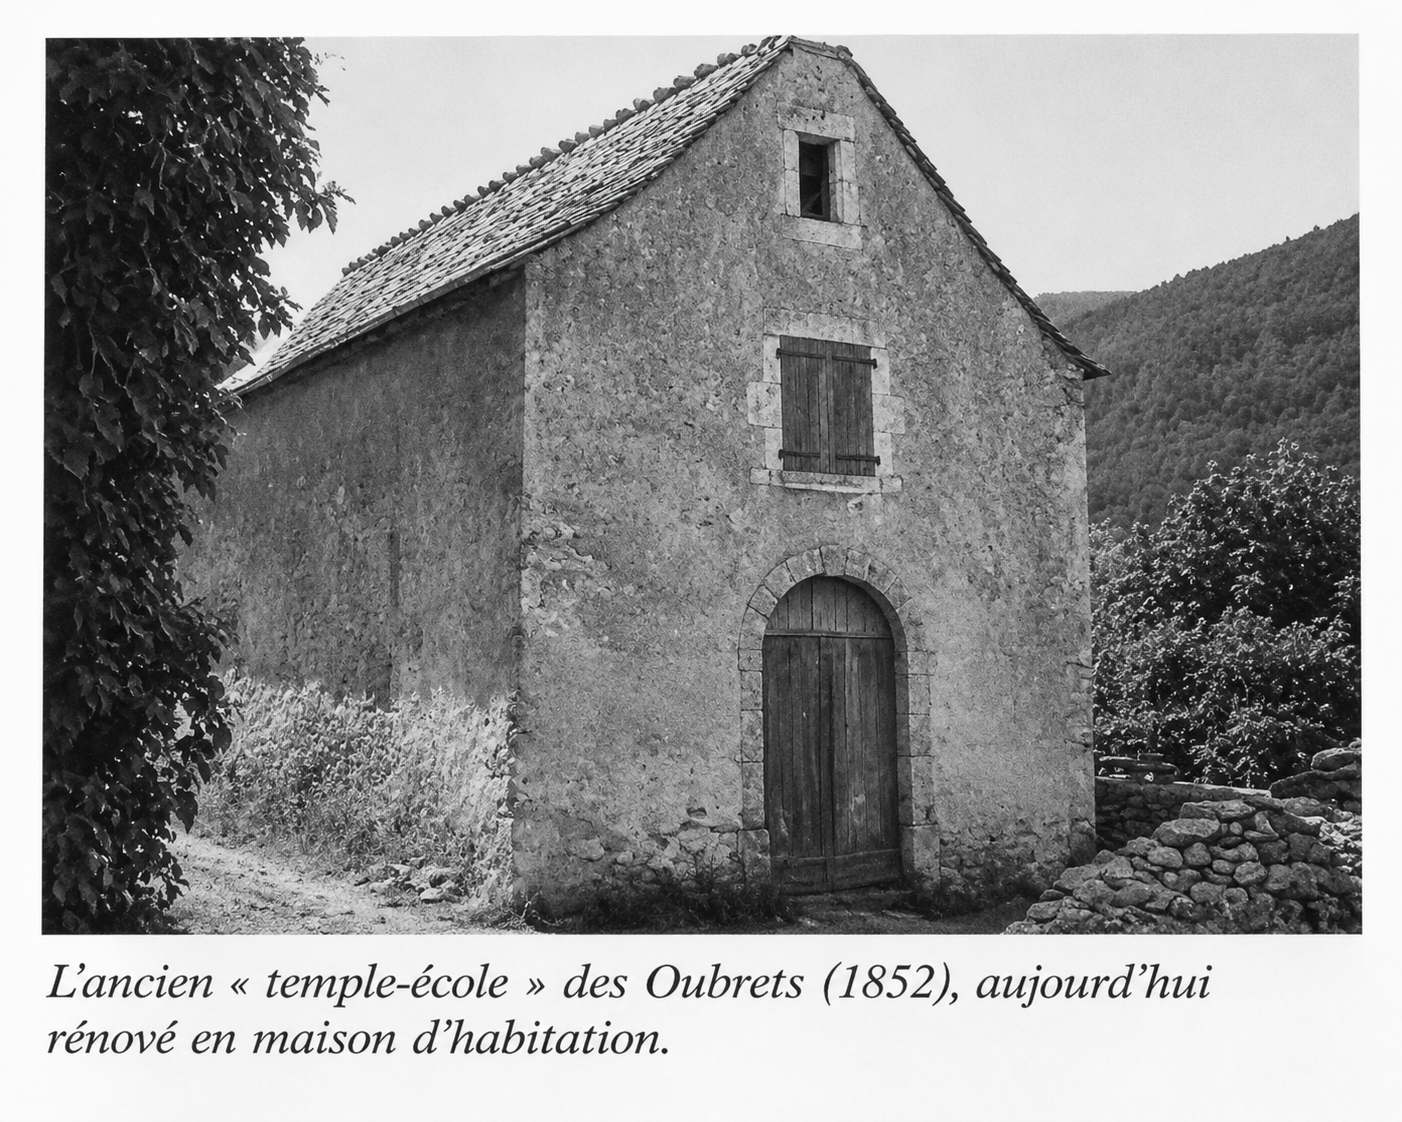
\includegraphics[width=0.38\textwidth]{imgs/116}
    
    \caption{\textit{L’ancien « temple-école » des Oubrets (1852), aujourd’hui
    rénové en maison d’habitation.}}
\end{figure}
